\documentclass[12pt]{article}

\newcommand{\CiteMathPackage}{../../math}
\newcommand{\CiteReference}{../reference.bib}

% Packages
\usepackage{setspace,geometry,fancyvrb,rotating}
\usepackage{marginnote,datetime,enumitem}
\usepackage{titlesec,indentfirst}
\usepackage{amsmath,amsfonts,amssymb,amsthm,mathtools}
\usepackage{threeparttable,booktabs,adjustbox}
\usepackage{graphicx,epstopdf,float,soul,subfig}
\usepackage[toc,page]{appendix}
\usdate

% Page Setup
\geometry{scale=0.8}
\titleformat{\paragraph}[runin]{\itshape}{}{}{}[.]
\titlelabel{\thetitle.\;}
\setlength{\parindent}{10pt}
\setlength{\parskip}{10pt}
\usepackage{Alegreya}
\usepackage[T1]{fontenc}

%% Bibliography
\usepackage{natbib,fancybox,url,xcolor}
\definecolor{MyBlue}{rgb}{0,0.2,0.6}
\definecolor{MyRed}{rgb}{0.4,0,0.1}
\definecolor{MyGreen}{rgb}{0,0.4,0}
\definecolor{MyPink}{HTML}{E50379}
\newcommand{\highlightR}[1]{{\emph{\color{MyRed}{#1}}}} 
\newcommand{\highlightB}[1]{{\emph{\color{MyBlue}{#1}}}}
\newcommand{\highlightP}[1]{{\emph{\color{MyPink}{#1}}}}
\usepackage[bookmarks=true,bookmarksnumbered=true,colorlinks=true,linkcolor=MyBlue,citecolor=MyRed,filecolor=MyBlue,urlcolor=MyGreen]{hyperref}
\bibliographystyle{econ}

%% Theorem Environment
\theoremstyle{definition}
\newtheorem{assumption}{Assumption}
\newtheorem{definition}{Definition}
\newtheorem{theorem}{Theorem}
\newtheorem{proposition}{Proposition}
\newtheorem{lemma}[theorem]{Lemma}
\newtheorem{example}{Example}
\newtheorem{corollary}[theorem]{Corollary}
\usepackage{mathtools}
\usepackage{\CiteMathPackage}

\begin{document}

%??%??%??%??%??%??%??%??%??%??%??%??%??%??%??%??%??%??%??%??%??%??
%?? title
%??%??%??%??%??%??%??%??%??%??%??%??%??%??%??%??%??%??%??%??%??%??

\title{\bf Skills, Tasks and Technologies: Implications for Employment and Earnings, Handbook of Labor Economics, 2011}
\author{Wenzhi Wang \thanks{This note is written in my pre-doc period at the University of Chicago Booth School of Business.} } 
\date{\today}
\maketitle

\citet{acemogluSkillsTasksTechnologies2011}

%??%??%??%??%??%??%??%??%??%??%??%??%??%??%??%??%??%??%??%??%??%??
%?? section 1. New Empirical Regularities
%??%??%??%??%??%??%??%??%??%??%??%??%??%??%??%??%??%??%??%??%??%??

\section{New Empirical Regularities} \label{sec_empicial_regularities}

The following are a number of central empirical findings about American labor market trends in the last three decades: 
\begin{itemize}[topsep=0pt, leftmargin=30pt, itemsep=0pt]
	\setlength{\parskip}{8pt} 
	\item Low skill (particularly low skill male) workers have experienced significant real earnings declines over the last four decades.
	\item There have been notably non-monotone changes in earnings levels across the earnings distribution over the last two decades (sometimes referred to as wage ``polarization''), even as the overall ``return to skill'' as measured by the college/high school earnings gap has monotonically increased.
	\item These changes in wage levels and the distribution of wages have been accompanied by systematic, non-monotone shifts in the composition of employment across occupations, with rapid simultaneous growth of both high education, high wage occupations and low education, low wage occupations in the United States and the European Union.
	\item This ``polarization'' of employment does not merely reflect a change in the composition of skills available in the labor market but also a change in the allocation of skill groups across occupations--and, in fact, the explanatory power of occupation in accounting for wage differences across workers has significantly increased over time.
	\item Recent technological developments and recent trends in offshoring and outsourcing appear to have directly replaced workers in certain occupations and tasks.
\end{itemize}

% {\bf Data}: the March Current Population Survey (March CPS), the combined Current Population Survey May and Outgoing Rotation Group samples (May/ORG CPS), the Census of Populations (Census), and the American Community Survey (ACS). 
% \footnote{The authors use the March files from 1964 to 2009 (covering earnings from 1963 to 2008) to form a sample of real weekly earnings for workers aged 16 to 64 who participate in the labor force on a full-time, full-year (FTFY) basis, defined as working 35-plus hours per week and 40-plus weeks per year. They also complement the March FTFY series with data on hourly wages of all current labor force participants using May CPS samples for 1973 through 1978 and CPS Outgoing Rotation Group samples for 1979 through 2009 (CPS May/ORG). To analyze levels and changes in occupational structure within and across detailed demographic groups, they exploit the 1960, 1970, 1980, 1990 and 2000 Census of Populations and the 2008 American Community Survey (ACS).}


%??%??%??%??%??%??%??%??%??%??%??%??%??%??%??%??%??%??%??%??%??%??
%?? section 2. The Canonical Model
%??%??%??%??%??%??%??%??%??%??%??%??%??%??%??%??%??%??%??%??%??%??

\section{The Canonical Model}
Most economic analyses of changes in wage structure and skill differentials build on the ideas proposed in \citet{katzChangesRelativeWages1992, cardCanFallingSupply2001}, among many others. In this strand of literature, \highlightB{the college/high school log wage ratio} serves as a summary index of the premium that high skill workers command relative to low skill workers, and this premium is determined by the relative supply and relative demand for skills. 

This literature interprets what has been observed by the data using the following reasoning: The relative demand for skills increases over time because changes in technology are assumed to be ``skill biased,'' in the sense that new technologies have greater skill demands for or are more complementary to high skill workers. Since relative supply has also steadily increased over the last century and a half, both because of the greater public investments in schooling and because of greater willingness of families and individuals to acquire schooling, this leads to Tinbergen's famous race between technology and the supply of skills. 

\subsection{The Simple Theory of the Canonical Model}

In the canonical model, there are two skills, high ($H$) and low ($L$). It draws no distinction between skills and occupations (tasks), so that high skill workers effectively work in separate occupations and perform different tasks from low skill workers. Critical to the two-factor model is that high and low skill workers are imperfect substitutes in production. The elasticity of substitution between these two skill types is central to understanding how changes in relative supplies affect skill premia. 

Suppose that the total supply of low skill labor is $L$ and the total supply of high skill labor is $H$. Naturally not all low (or high) skill workers are alike in terms of their marketable skills. As a simple way of introducing this into the canonical model, suppose that each worker is endowed with either high or low skill, but there is a distribution across workers in terms of efficiency units of these skill types. In particular, let $\Lc$ denote the set of low skill workers and $\Hc$ denote the set of high skill workers. Each low skill worker $i \in \Lc$ has $l_i$ efficiency units of low skill labor and each high skill worker $i \in \Hc$ has $h_i$ units of high skill labor. All workers supply their efficiency units inelastically. Thus the total supply of high skill and low skill labor in the economy can be written as:
$$
L=\int_{i \in \mathcal{L}} l_i d i \quad \text { and } \quad H=\int_{i \in \mathcal{H}} h_i d i .
$$

The production function for the aggregate economy takes the following constant elasticity of substitution form \footnote{This production function is typically written as $Y = \bs{\g\bp{A_L L}^{\frac{\s - 1}{\s}} + \bp{1-\g}\bp{A_H H}^{\frac{\s - 1}{\s}}}^{\frac{\s}{\s - 1}}$, where $\g$ is the distribution parameter. To simplify notation, we suppress $\g$ (i.e., set if equal to $1/2$).}
\begin{equation}
    \label{canonical_model_production_function}
    Y = \bs{\bp{A_L L}^{\frac{\s - 1}{\s}} + \bp{A_H H}^{\frac{\s - 1}{\s}}}^{\frac{\s}{\s - 1}},
\end{equation}
where $\s \in [0, \infty)$ is the elasticity of substitution between high and low skill labor, and $A_L$ and $A_H$ are factor-augmenting technology terms. 

\highlightP{Need more calculation here about the production function!}

The elasticity of substitution between high and low skill workers plays a pivotal role in interpreting the effects of different types of technological changes in this canonical model. We refer to high and low skill workers as \highlightB{gross substitutes} when the elasticity of substitution $\s > 1$, and \highlightB{gross complements} when $\s < 1$. Three focal cases are: (i) $\s \rightarrow 0$, when high skill and low skill workers will be Leontief, and output can be produced only by using high skill and low skill workers in fixed portions; (ii) $\s \rightarrow \infty$ when high skill and low skill workers are perfect substitutes (and thus there is only one skill, which $H$ and $L$ workers possess in different quantities), and (iii) $\s \rightarrow 1$, when the production function tends to the Cobb-Douglas case. 

In this framework, technologies are \highlightB{factor-augmenting}, meaning that technological change serves to either increase the productivity of high or low skill workers (or both). This implies that there are no explicitly skill replacing technologies. However, the lack of directly skill replacing technologies in the canonical model is an important reason why it does not necessarily provide an entirely satisfactory framework for understanding changes in the earnings and employment distributions over the last four decades in US. 

The production function (\ref{canonical_model_production_function}) admits three different interpretations.
\begin{enumerate}[topsep=0pt, leftmargin=20pt, itemsep=0pt, label=(\arabic*)]
\setlength{\parskip}{10pt} 

\item There is only one good, and high skill and low skill workers are imperfect substitutes in the production of this good. 

\item It is equivalent to an economy where consumers have utility function $\left[Y_l^{\frac{\sigma-1}{\sigma}}+Y_h^{\frac{\sigma-1}{\sigma}}\right]^{\frac{\sigma}{\sigma-1}}$ defined over two goods. Good $Y_h$ is produced using only high skill workers, and $Y_l$ using only low skill workers, with production functions $Y_h = A_H H$, and $Y_l = A_L L$.

\item A mixture of the above two whereby different sectors produce goods that are imperfect substitutes, and high and low education workers are employed in both sectors.
\end{enumerate}

Since labor markers are competitive, the low skill unit wage is simply given by the value of marginal product of low skill labor, which is obtained by differentiating (\ref{canonical_model_production_function}) as 
\begin{equation}
    \label{canonical_model_low_skill_wage}
    w_L = \frac{\partial Y}{\partial L} = A_L^{\frac{\s - 1}{\s}} \bs{A_L^{\frac{\s - 1}{\s}} + A_H^{\frac{\s - 1}{\s}} \bp{\frac{H}{L}}^{\frac{\s - 1}{\s}} }^{\frac{1}{\s - 1}}.
\end{equation}
Given this unit of wage, the earnings of worker $i \in \Lc$ is simply 
$$W_i = w_L l_i .$$

There are two important implications of Equation (\ref{canonical_model_low_skill_wage}):
\begin{enumerate}[topsep=0pt, leftmargin=20pt, itemsep=0pt, label=(\arabic*)]
\setlength{\parskip}{10pt} 
\item $\pdfrac{w_L}{\bp{\frac{H}{L}}} > 0$, that is, as the fraction of high skill workers in the labor force increases, the low skill wage should increase. This is an implication of imperfect substitution between high and low skill workers. An increase in the fraction (or relative supply) of high skill workers increases the demand for the services of low skill workers, pushing up their unit wage.
\item $\pdfrac{w_L}{A_L} > 0$ and $\pdfrac{w_L}{A_H} > 0$, that is, either kind of factor-augmenting technical change \highlightP{increases} wages of low skill workers (except in the limit case where $\s = \infty$, the second inequality is weak). This result is intuitive but will also turn out to be important: technological improvements of any sort will lead to higher wages for both skill groups in the canonical model. Thus unless there is ``technical regress'', the canonical model cannot account for declining real wages of a factor whose supply is not shifting outward.
\end{enumerate}

Similarly, the high skill unit wage is
\begin{equation}
    \label{canonical_model_high_sill_wage}
    w_H=\frac{\partial Y}{\partial H}=A_H^{\frac{\alpha-1}{\sigma}}\left[A_L^{\frac{\alpha-1}{\sigma}}(H / L)^{-\frac{\sigma-1}{\sigma}}+A_H^{\frac{\alpha-1}{\sigma}}\right]^{\frac{1}{\sigma-1}} .
\end{equation}
We again have similar comparative statics. First, $\pdfrac{w_H}{\bp{\frac{H}{L}}} < 0$, so that when high skill workers become more abundant, their wages should fall. Second, $\pdfrac{w_H}{A_L} > 0$ and $\pdfrac{w_H}{A_H} > 0$, so that technological progress of any kind increases high skill (as well as low skill) wages.

It can also be verified that an increase in either $A_L$ or $A_H$ (and also an increase in $H/L$) will raise average wages in this model.

Combining (\ref{canonical_model_low_skill_wage}) and (\ref{canonical_model_high_sill_wage}), the skill premium -- the unit high skill wage divided by the unit low skill wage -- is 
\begin{equation}
    \label{canonical_model_skill_premium}
    \o = \frac{w_H}{w_L} = \bp{\frac{A_H}{A_L}}^{\frac{\s-1}{\s}} \bp{\frac{H}{L}}^{-\frac{1}{\s}}.
\end{equation}
Equation (\ref{canonical_model_skill_premium}) can be rewritten in a more convenient form by taking logs, 
\begin{equation}
    \label{canonical_model_log_skill_premium}
    \ln \omega=\frac{\sigma-1}{\sigma} \ln \left(\frac{A_H}{A_L}\right)-\frac{1}{\sigma} \ln \left(\frac{H}{L}\right) .
\end{equation}

Equation (\ref{canonical_model_log_skill_premium}) shows that there is a simple log linear relationship between the skill premium and the relative supply of skills as measured by $H/L$:
\begin{equation}
    \label{canonical_model_skill_premium_over_supply}
    \pdfrac{\ln \o}{\ln \of{\frac{H}{L}}} = - \frac{1}{\s} < 0.
\end{equation}
This relationship corresponds to the second of the two forces in Tinbergen's race (the first being technology, the second being the supply of skills): for a given skill bias of technology, captured here by $A_H / A_L$, an increase in the relative supply of skills reduces the skill premium with an elasticity of $\frac{1}{\s}$.

Interpretation: An increase in $H/L$ creates two different types of substitution. 

First, if high and low skill workers are producing different goods, the increase in high skill workers will raise output of the high skill intensive good, leading to a substitution towards the high skill good in consumption. This substitution hurts the relative earnings of high skill workers since it reduces the relative marginal utility of consumption, and hence the real price, of the high skill good. 

Second, when high and low skill workers are producing the same good but performing different functions, an increase in the number of high skill workers will necessitate a substitution of high skill workers for the functions previously performed by low skill workers. The downward sloping relationship betwen relative supply and the skill premium implies that if technology, in particular $A_H / A_L$, had remained roughly constant over recent decades, the remarkable increase in the supply of skills would have led to a significant decline in the skill premium. The lack of such a decline is a key reason why economists believe that the first force in Tinbergen's race -- changes in technology increasing the demand for skills -- must have also been important throughout the 20th century. 

More formally, differentiating (\ref{canonical_model_log_skill_premium}) with respect to $A_H / A_L$ yields:
\begin{equation}
    \label{canonical_model_skill_premium_over_tech}
    \pdfrac{\ln \o}{\ln \bp{\frac{A_H}{A_L}}} = \frac{\s - 1}{\s}.
\end{equation}
Equation (\ref{canonical_model_skill_premium_over_tech}) implies that if $\s > 1$, then relative improvements in the high skill augmenting technology (i.e., in $A_H / A_L$) increase the skill premium. This can be seen as a shift out of the relative demand curve for skills. The converse is obtained when $\s < 1$: relative improvements in the high skill augmenting technology shift the relative demand cure inward and reduces the skill premium.

This appears paradoxical at first, but is in fact quite intuitive. Consider, for example, how factor-augmenting technology change affects the wages of the augmented factor when the production function is Leontief (fixed proportions). In this case, as $A_H$ increases, high skill workers become more productive, and hence the demand for low skill workers increases by more than the demand for high skill workers. Effectively, the increase in $A_H$ creates ``excess supply'' of high skill workers given the number of low skill workers, which depresses the high skill relative wage. This observation raises an important caveat. It is tempting to interpret improvements in technologies used by high skill workers, $A_H$, as ``skill biased''. However, when the elasticity of substitution is less than $1$, it will be advances in technologies used with low skill workers, $A_L$, that increase the relative productivity and wages of high skill workers, and an increase in $A_H$ relative to $A_L$ will be ``skill replacing''. Nevertheless, the conventional wisdom is that the skill premium increases when high skill workers become relatively more -- not relatively less -- productive, which is consistent with $\s > 1$.

\subsection{Brining Tinbergen's Education Race to the Data}

The key equation of the canonical model, (\ref{canonical_model_log_skill_premium}), links the skill premium to the relative supply of skills, $H/L$, and to the relative technology term, $A_H / A_L$. This last term is not directly observed. Nevertheless, we can make considerable empirical progress by taking a specific form of Tinbergen;s hypothesis, and assuming that there is a log linear increase in the demand for skills over time coming from technology, captured in the following equation:
\begin{equation}
    \label{canonical_model_empirical_assumption}
    \ln \of{\frac{A_{H,t}}{A_{L,t}}} = \g_0 + \g_1 t,
\end{equation}
where $t$ is calendar time and variables written with $t$ subscript refer to these variables at time $t$. Substituting this equation into (\ref{canonical_model_log_skill_premium}), we obtain, 
\begin{equation}
    \label{canonical_model_regression_equation}
    \ln \omega_t=\frac{\sigma-1}{\sigma} \gamma_0+\frac{\sigma-1}{\sigma} \gamma_1 t-\frac{1}{\sigma} \ln \left(\frac{H_t}{L_t}\right) .
\end{equation}

Equation (\ref{canonical_model_regression_equation}) implies that ``technological developments'' take place at a constant rate, while the supply of skilled workers may grow at varying rates at different points in time. Therefore, changes in the skill premium will occur when the growth rate of the supply of skills differ from the pace of technological progress. In particular, when $H/L$ grows faster than the rate of skill biased technical change, $\bp{\s-1}\g_1$, the skill premium will fall. And when the supply growth falls short of this rate, the skill premium will increase. 

The seminal work of \citet{katzChangesRelativeWages1992} demonstrated the power of the approach outlined above by fitting Equation (\ref{canonical_model_regression_equation}) to aggregate time-series data on college/high school relative wages and college/high school relative supplies for the years 1963 through 1987. The main implication is shown in Figure \ref{fig_KatzMurphy_predictions}:
\begin{figure}[H]
    \noindent\caption{Katz-Murphy prediction model for the college-high school wage gap.}
    \begin{center}
        \resizebox{0.7\textwidth}{!}{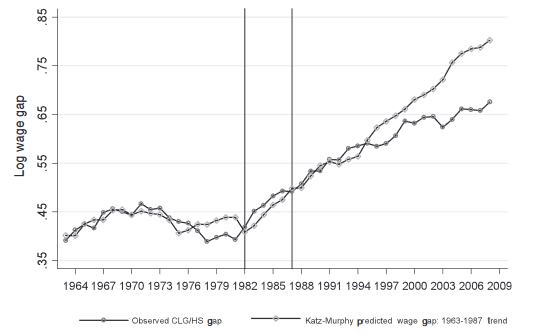
\includegraphics{HLE_KatzMurphy_predictions.png}}
        \label{fig_KatzMurphy_predictions}
    \end{center}
\end{figure}
The fit of the model remains quite good through the year 1992,five years out of sample. But the model systematically deviates from the data thereafter, predicting a sharper rise in the college premium than actually occurs. If we free up the linear time trend with somewhat richer specifications: a linear spline, allowing the time trend to deviate from its initial trajectory after 1992; a quadratic time trend; and a cubic time trend. When fit to the data, all three of these variants suggest a significant deceleration in trend relative demand takes place sometime during the 1990s. Thus, \highlightP{taken at face value}, this model suggests that relative demand for college workers decelerated in the 1990s, which does not accord with common intuitions regarding the nature or pace of technological changes occurring in this era. 

One can gain additional identification and explanatory power with this model by considering a slightly richer set of facts. In reality, changes in the college/high school wage gap have differed substantially by age/experience groups over recent decades. This pattern may be seen through a comparison of the college premium for younger workers (those with 0-9 years of potential experience) and older workers (those with 20-29 years of potential experience). These facts may better accord with a simple extension to the canonical model. To the extent that workers with similar education but with different ages or experience levels are imperfect substitutes in production, one would expect age-group or cohort-specific relative skill supples -- as well as aggregate relative skill supplies -- to affect the evolution of the college/high school premium by age or experience, as emphasized by \citet{cardCanFallingSupply2001}. 

\subsection{Overall Inequality in the Canonical Model} 

Our brief overview of the salient empirical patterns in Secion \ref{sec_empicial_regularities} highlights that there have been rich and complex changes in the overall earning distribution over the last four decades. While changes in the college premium (or more generally in the returns to different levels of schooling) have contributed to these changes in the earnings distribution, there have also been significant changes in inequality among workers with the same education -- i.e., \highlightP{within-groups} as well as \highlightP{between groups}.

In the canonical model, the within-group wage difference is invariant to skill prices and thus changes in overall inequality will closely mimic changes in the skill premium. In particular, recall that all workers in the set $\Lc$ and $\Hc$ always face the same skill price. Therefore, changes in the skill premium should have no direct effect on within group inequality, Mathematically, in this model the relative earnings of two workers in the same group, say $\Lc$, is given by 
\begin{equation}
    \label{canonical_model_within_group_diff}
    \frac{W_i}{W_{i^\prime}} = \frac{w_L l_i}{w_L l_{i^\prime}} = \frac{l_i}{l_{i^\prime}}, \text{ for  } i, i^\prime \in \Lc .
\end{equation}
In this simple form, the canonical model can exhibit significant within group wage inequality, but inequality will be independent of the skill premium.

Naturally, this feature can be changed by positing that there are increasing returns to efficiency units of skill, so when the relative demand for high skill labor increases, this increases the demand for ``more skilled'' college graduates by relatively more than for ``less skilled'' college graduates. \highlightP{One way to incorporate this idea is to extend the canonical model by drawing a distinction between observable groups (such as college vs. non-college) and skills.} 

For example, we can remain fairly close to the spirit of the canonical model and continue to assume that there are only two skills, but now suppose that these skills are only imperfectly proxied by education. Specifically, we can assume that the two observable groups are college and non-college, and a fraction $\f_c$ of college graduates are high skill, while a fraction $\f_n < \f_c$ of non-college graduates are high skill (the remaining fractions in both groups being low skill as usual). Let us again denote the skill premium by $\o = w_H / w_L$. This is no longer the college premium, i.e., the ratio of average college ($w_C$) to non-college wages ($w_C$). Instead, 
$$
\omega^c=\frac{w_C}{w_N}=\frac{\phi_c w_H+\left(1-\phi_c\right) w_L}{\phi_n w_H+\left(1-\phi_n\right) w_L}=\frac{\phi_c \omega+\left(1-\phi_c\right)}{\phi_n \omega+\left(1-\phi_n\right)} .
$$

It is straightforward to verify that, because $\f_n < \f_c$, this college premium is increasing in $\o$, so that when the true price of skill increases, the observed college premium will also rise. In addition, we can define within group inequality in this context as the ratio of the earnings of high wage college graduates (or non-college graduates) to that of low wage college graduates (or non-college graduates). Given our assumptions, we also have $\o^{\text{within}} = \o$ (since high wage workers in both groups earn $w_H$, while low wage workers earn $w_L$). As long as $\f_c$ and $\f_n$ remain constant, $\o^c$ and $\o^{\text{within}}$ will move together. Therefore in this extended version of the canonical model, an increase in the returns to observed skills -- such as education -- will also be associated with an increase in the returns to unobserved skills. Moreover, we can also think of large changes in relative supplies being associated with compositional changes, affecting $\f_c$ and $\f_n$, so within group inequality can change differently than the skill premium, and thus overall inequality can exhibit more complex changes as supplies and technology evolve.

This model thus provides a useful starting point for thinking about changes in within group inequality and the overall earnings distribution, and linking them both to the market price of skills. In light of this model, the increase in the overall earnings inequality starting in the late 1970s or early 1980s is intimately linked to the increase in the demand for skills, also reflected in the increase in the college premium. While this parsimonious framework is valuable for analyzing the evolution of distribution of earnings, it does not provide sufficient nuance for understanding why different parts of the earnings distribution move differently and moreover, do so markedly during different time periods. 

\subsection{Endogenous Changes in Technology}

The canonical model is most powerful as an empirical framework when skill biased technical change can be approximated by a steady process, such as the (log) linear trend posited in (\ref{canonical_model_empirical_assumption}). However, the discussion in \citet{autorComputingInequalityHave1998} suggests that the pace of skill biased technical change was likely more rapid between 1970 and 1990 than between 1940 and 1970. The evidence discussed above, on the other hand, suggests that the pace of skill biased technical change slowed during the 1990s, at least viewed through the lens of the canonical model.

But once we recognize that skill biased technical change is not a steady process, it becomes more important to understand when we should expect it to be more rapid and when we should expect it not to take place at all. The canonical model is silent on this question. \citet{acemogluWhyNewTechnologies1998} suggests that modelling the endogenous response of the skill bias of technology might generate richer insights. In particular, under relatively general conditions, models of endogenous (directed) technical change imply that technology should become more skill biased following increases in the supply of high skill workers. According to this perspective, steady skill biased technical change might be partly a response to the steady increase in the supply of skills during the past century (thus uniting the two parts of Tinbergen;s race).

%??%??%??%??%??%??%??%??%??%??%??%??%??%??%??%??%??%??%??%??%??%??
%?? section 3. The Task-Based Model
%??%??%??%??%??%??%??%??%??%??%??%??%??%??%??%??%??%??%??%??%??%??

\section{The Task-Based Model}

Many of the shortcomings of the canonical model can, we believe, be addressed by incorporating a clear distinction between workers' skills and job tasks and allowing the assignment of skills to tasks to be determined in equilibrium by labor supplies, technologies, and task demands. In this terminology, a \highlightB{task} is a unit of work activity that produces output (goods and services). A \highlightB{skill} is a worker's \highlightP{endowment} of capabilities for performing various tasks. This endowment is a stock, which may be either exogenously given or acquired through schooling and other investments. Workers apply their skill endowments that skills are applied to produce output -- skills do not directly produce output. Task models provide a natural framework for interpreting patterns related to occupations in the labor market, since we can think of occupations as bundles of tasks. In this light, the canonical model may be seen as a special case of the general task-based model in which there is a one-to-one mapping between skills and tasks. 

The distinction between skills and tasks becomes particularly relevant when \highlightB{workers of a given skill level can perform a variety of tasks and, moreover, can change the set of tasks that they perform in response to changes in labor market conditions and technology}.

This model is a generalization of \citet{acemogluProductivityDifferences2001} and is also related to \citet{costinotMatchingInequalityWorld2010}. Given the central role that the comparative advantage differences across different types of workers play in our model, we refer to it as a \highlightB{Ricardian model of the labor market}.

\subsection{Environment}

We consider a static environment with a unique final good. For now, the economy is closed and there is no trade in tasks. The unique final good is produced by combining a continuum of tasks represented by the unit interval, $\bs{0,1}$. We simplify the analysis by assuming a Cobb-Douglas technology mapping services of this range of tasks to the final good. In particular, 
\begin{equation} 
    \label{task_model_good_production}
	Y = \exp\of{\int_0^1 \ln\of{y\of{i}} di}, 
\end{equation}
where $Y$ denotes the output of a unique final good and we will refer to $y\of{i}$ as the ``service'' or production level of task. We will also alternately refer to workers ``performing'' or producing a task. We assume that all markets are competitive. Throughout, we choose the price of the final good as the numeraire.
\footnote{
    More generally, in \citet{autorTaskApproachLabor2013}, the production function is defined as 
    \begin{equation}
        \notag
        Y=\bs{\int_0^1 y\of{i}^{\frac{\eta-1}{\eta}} d i}^{\frac{\eta}{\eta-1}},
    \end{equation}
    where $\eta$ is the elasticity of substitution between tasks.
}

There are three factors of production, high, medium, and low skilled workers. In addition, we will introduce capital or technology below. We first assume that there is a fixed, inelastic supply of the three types of workers, $L, M$, and $H$. We return to the supply response of different types of skills to changes in technology later. 

Each task has the following production function
\begin{equation} 
    \label{task_model_task_production}
	y\of{i} = A_L \alpha_L\of{i} l\of{i} + A_M \alpha_M\of{i} m\of{i} + A_H \alpha_H\of{i} h\of{i} + A_K \alpha_K\of{i} k\of{i},
\end{equation}
where $A$ terms represent factor-augmenting technology, and $\alpha_L\of{i}, \alpha_M\of{i}, \alpha_H\of{i}$ are the task productivity schedules, designating the productivity of {low, medium and high skill} workers in different tasks. For example, $\alpha_L\of{i}$ is the productivity of low skill workers in task $i$, and $l\of{i}$ is the number of low skill workers allocated to task $i$. It is critical to observe that this production function for task services implies that each task can be performed by low, medium or high skill workers, but \highlightP{the comparative advantage of skill groups differ across tasks, as captured by the $\a$ terms}. These differences in comparative advantage will play a central role in our model.

We impose the following assumption on the structure of comparative advantage throughout:
\begin{assumption} \label{task_model_ass_comparative_advantage}
	$\frac{\a_L\of{i}}{\a_M\of{i}}$ and $\frac{\a_M\of{i}}{\a_H\of{i}}$ are continuously differentiable and strictly decreasing.
\end{assumption}
This assumption specifies the structure of comparative advantage in the model. It can be interpreted as stating that \highlightB{higher indices correspond to ``more complex'' tasks in which high skill workers are better than medium skill workers and medium skill workers are better than low skill workers}. Though not very restrictive, this assumption ensures a particularly simple and tight characterization of equilibrium in this economy.

Factor market clearing requires
\begin{equation}
    \label{task_model_market_clearing}
	\int_0^1 l\of{i} d i \leq L, \quad \int_0^1 m\of{i} d i \leq M \quad \text { and } \quad \int_0^1 h\of{i} d i \leq H .
\end{equation}

When we introduce capital, we will assume that it is available at some constant price $r$.

\subsection{Equilibrium without Machines}

An equilibrium is defined in the usual manner as an allocation in which (final good) producers maximize profits and labor markets clear. For now, there no labor supply decision on the part of the workers.

\subsubsection{Allocation of Skills to Tasks}

The characterization of equilibrium in this economy is simplified by the structure of comparative advantage differences in Assumption \ref{task_model_ass_comparative_advantage}. In particular, there will exist some $I_L$ and $I_H$ such that all tasks $i < I_L$ will be performed by low skill workers, and all tasks $i > I_H$ will be performed by high skill workers. Intermediate tasks will be performed by medium skilled workers. We can think of these intermediate tasks as the routine tasks performed by workers in many production, clerical, and administrative support occupations. More formally, we have:
\begin{lemma} \label{task_model_lemma1}
	In any equilibrium there exist $I_L$ and $I_H$ such that $0 < I_L < I_H < 1$ and for any $i < I_L , m\of{i} = h \of{i} = 0$, for any $i \in \bs{I_L , I_H}, l \of{i} = h \of{i} = 0$, and for any $i > I_H , l\of{i} = m\of{i} = 0$.
\end{lemma}

This lemma shows that the set of tasks will be partitioned into three (convex) sets, one performed by low skill workers, one performed by medium skill workers and one performed by high skill workers. Crucially, the boundaries of these sets, $I_L$ and $I_H$, are endogenous and will respond to changes in skill supplies and technology. This introduces the first type of substitution that will play an important role in our model: \highlightP{the substitution of skills across tasks}. Given the types of skills supplied in the market, firms (equivalently workers) will optimally choose which tasks will be performed by which skill groups.

\subsubsection{The Law of One Price for Skills}

Even though workers of the same skill level perform different tasks, in equilibrium they will receive the same wage -- a simple ``law of one price'' that has to hold in any competitive equilibrium. We now derive these prices.

Let $p\of{i}$ denote the price of services of task $i$. Since we chose the final good as numeraire (setting its price to $1$), We have
\begin{equation}
	\notag
	\exp\of{\int_0^1 \ln\of{p\of{i}} di} = 1.
\end{equation}

In any equilibrium, all tasks employing low skill workers must pay them the same wage, $w_L$, since otherwise, given the competitive market assumption, no worker would supply their labor to tasks paying lower wages. Similarly, all tasks employing medium skill workers must pay a wage $w_M$, and all tasks employing high skill workers must pay a wage $w_H$. As a consequence, the value marginal product of all workers in a skill group must be the same in all the tasks that they are performing. In particular, in view of Lemma and \ref{task_model_lemma1} and the production function (\ref{task_model_task_production}), this implies:
\begin{equation}
	\notag
	\begin{cases}
		w_L = p\of{i}A_L\a_L\of{i}, & \text{for any } i < I_L \\
		w_M = p\of{i}A_M\a_M\of{i}, & \text{for any } I_L < i < I_H \\
		w_H = p\of{i}A_H\a_H\of{i}, & \text{for any } i > I_H
	\end{cases}
\end{equation}

This observation has a convenient implication. We must have that the price difference between any two tasks produced by the same type of worker must exactly offset the productivity difference of this type of worker in these two tasks. For example, for low skill workers we have
\begin{equation} 
    \label{task_model_price_index_for_low_skill}
	p\of{i} \a_L\of{i} = p\of{i^\prime} \a_L\of{i^\prime} \equiv P_L,
\end{equation}
for any $i, i^\prime < I_L$, where the last equality defines $P_L$ as the price ``index'' of tasks performed by low skill workers. Note, however, that this price is endogenous not only because of the usual supply-demand reasons, but also because the set of tasks performed by low skill workers is endogenously determined. Similarly, we have 
\begin{equation} 
    \label{task_model_price_index_for_medium_skill}
	p\of{i} \a_M\of{i} = p\of{i^\prime} \a_M\of{i^\prime} \equiv P_M, \text{for any } I_L < i, i^\prime < I_H
\end{equation}
\begin{equation} 
    \label{task_model_price_index_for_high_skill}
	p\of{i} \a_H\of{i} = p\of{i^\prime} \a_H\of{i^\prime} \equiv P_H, \text{for any } i, i^\prime > I_H
\end{equation}

The Cobb-Douglas technology (the unitary elasticity of substitution between tasks) in (\ref{task_model_good_production}) implies that ``expenditure'' across all tasks should be equalized, and given our choice of numeraire, this expenditure should be equal to the value of total output. More specifically, the first-order conditions for cost minimization in the production of the final good imply that $p\of{i} = y\of{i} = p\of{i^\prime} y\of{i^\prime}$ for any $i, i^\prime$. Alternatively, using our choice of the final good as numeraire, we can write 
\begin{equation} 
    \label{task_model_cost_minimization}
	p\of{i} y\of{i} = Y \; \text{ for any } i \in \bp{0, 1}.
\end{equation}
(In particular, note that the ideal price index for the final good, $P$, is defined such that $y\of{i}/ Y = p\of{i}/P$, and our choice of numeraire implies that $P=1$, which gives (\ref{task_model_cost_minimization})).

Now consider two tasks $i, i^\prime < I_L$ (performed by low skill workers), then using the definition of the productivity of low skill workers in these tasks, we have 
\begin{equation}
	\notag
	p\of{i} \a_L\of{i} l\of{i} = p\of{i^\prime} \a_L\of{i^\prime} l\of{i^\prime}.
\end{equation}
Therefore, we conclude that $l\of{i}=l\of{i^\prime}$, and using the market clearing condition for low skilled workers, we must have
\begin{equation}
    \label{task_model_labor_demand_for_low_skill}
	l\of{i} = \frac{L}{I_L} \text{for any } i < I_L.
\end{equation}
This is a very convenient implication of the Cobb-Douglas production structure. With a similar argument, we also have 
\begin{equation}
    \label{task_model_labor_demand_for_medium_skill}
	m\of{i} = \frac{M}{I_H - I_L} \text{for any } I_L < i < I_H.
\end{equation}
\begin{equation}
    \label{task_model_labor_demand_for_high_skill}
	h\of{i} = \frac{H}{1-I_H} \text{for any } i > I_H.
\end{equation}

The above expressions are derived by comparing expenditures on tasks performed by the same type of worker. Now comparing two tasks performed by high and medium skill workers ($I_L < i < I_H < i^\prime$), we obtain from (\ref{task_model_cost_minimization}) that $p\of{i}A_M\a_M\of{i}m\of{i}=p\of{i^\prime}A_H\a_H\of{i^\prime}h\of{i^\prime}$. Next using (\ref{task_model_price_index_for_medium_skill}) and (\ref{task_model_price_index_for_high_skill}), we have 
$$
\frac{P_M A_M M}{I_H - I_L} = \frac{P_H A_H H}{1 - I_H},
$$ 
or 
\begin{equation} 
    \label{task_model_price_index_ratio_h_over_m}
	\frac{P_H}{P_M}=\left(\frac{A_H H}{1-I_H}\right)^{-1}\left(\frac{A_M M}{I_H-I_L}\right),
\end{equation}
Similarly, comparing two tasks performed by medium and low skill workers, we obtain 
\begin{equation}
    \label{task_model_price_index_ratio_m_over_l}
	\frac{P_M}{P L}=\left(\frac{A_M M}{I_H-I_L}\right)^{-1}\left(\frac{A_L L}{I_L}\right) .
\end{equation}

\subsubsection{No Arbitrage across Skills}

The above derivations show that the key equilibrium objects of the model are the threshold tasks $I_L$ and $I_H$. These will be determined by a type of ``no arbitrage'' condition equalizing the cost of producing these threshold tasks using different skills. We now derive these no arbitrage conditions and determine the threshold tasks. 

Recall, in particular, that the threshold task $I_H$ must be such that it can be profitably produced using either high skilled or medium skilled workers. \highlightP{This is equivalent to task $I_H$ having the same equilibrium supply either when produced only with skilled or unskilled workers.} That is, it implies our first no arbitrage condition (between high and medium skills) is,
\begin{equation}
    \label{task_model_no_arbitrage_between_m_and_h}
	\frac{A_M \alpha_M\left(I_H\right) M}{I_H-I_L}=\frac{A_H \alpha_H\left(I_H\right) H}{1-I_H}
\end{equation}
With an analogous argument, we obtain the second no arbitrage condition as 
\begin{equation}
    \label{task_model_no_arbitrage_between_m_and_l}
	\frac{A_L \alpha_L\left(I_L\right) L}{I_L}=\frac{A_M \alpha_M\left(I_L\right) M}{I_H-I_L} .
\end{equation}

\subsubsection{Equilibrium Wages and Inequality}

Once the threshold tasks, $I_L$ and $I_H$, are determined, wage levels and earnings differences across skill groups can be found in a straightforward manner. In particular, wages are obtained simply as the values of the marginal products of different types of skills. For example, for low skill workers, this is:
\begin{equation}
    \label{task_model_wage_for_low_skill}
	w_L = P_L A_L .
\end{equation}

Equally, or perhaps even more, important than the level of wages are their ratios, which inform us about the wage structure an inequality. For example, comparing high and medium skill wages, we have 
$$
\frac{w_H}{w_M} = \frac{P_H A_H}{P_M A_M}.
$$
A more convenient way of expressing these is to use (\ref{task_model_no_arbitrage_between_m_and_h}) and write the relative wages simply in terms of relative supplies and the equilibrium allocation of tasks to skill groups, given by $I_L$ and $I_H$. That is,
\begin{equation}
    \label{task_model_wage_ratio_between_h_and_m} 
	\frac{w_H}{w_M} = \left(\frac{1-I_H}{I_H-I_L}\right)\left(\frac{H}{M}\right)^{-1} .
\end{equation}
Similarly, the wage of medium relative to low skill workers is given by
\begin{equation}
    \label{task_model_wage_ratio_between_m_and_l} 
	\frac{w_M}{w_L}=\left(\frac{I_H-I_L}{I_L}\right)\left(\frac{M}{L}\right)^{-1}.
\end{equation}
These expressions highlight the central role that allocation of tasks to skills plays in the model. Relative wages can be expressed simply as a function of relative supplies and equilibrium task assignments (in particular, the threshold tasks, $I_L$ and $I_H$).

These equations, together with the choice of the numeraire, $\int_0^1 \ln\of{p\of{i}} di = 0$, fully characterize the equilibrium. In particularly, using (\ref{task_model_price_index_for_low_skill})-(\ref{task_model_price_index_for_high_skill}), we can write the last equilibrium condition as:
\begin{equation} 
    \label{task_model_numeraire_condition}
	\int_0^{I_L}\left(\ln P_L-\ln \alpha_L(i)\right) d i+\int_{I_L}^{I_H}\left(\ln P_M-\ln \alpha_M(i)\right) d i + \int_{I_H}^1\left(\ln P_H-\ln \alpha_H(i)\right) d i=0 .
\end{equation}
Equations (\ref{task_model_wage_ratio_between_h_and_m}) and (\ref{task_model_wage_ratio_between_m_and_l}) give the relative wages of high to medium and medium to low skill workers. To obtain the wage \highlightB{level} for any one of these three groups, we need to use the price normalization in (\ref{task_model_numeraire_condition}) together with (\ref{task_model_price_index_ratio_h_over_m}) and (\ref{task_model_price_index_ratio_m_over_l}) to solve for one of the price indices, for example, $P_L$, and then (\ref{task_model_wage_for_low_skill}) will give $w_L$ and the levels of $w_M$ and $w_H$ can be readily obtained from (\ref{task_model_wage_ratio_between_h_and_m}) and (\ref{task_model_wage_ratio_between_m_and_l}).

{\bf Summary of equilibrium}

The next proposition summarizes our equilibrium characterization and highlights several important features of the equilibrium.
\begin{proposition}
    \label{task_model_prop1}
	There exists a unique equilibrium summarized by $\bp{I_L, I_H, P_L, P_M, P_H, w_L, w_M, w_H}$ given by Equations (\ref{task_model_price_index_ratio_h_over_m})-(\ref{task_model_numeraire_condition}).
\end{proposition}

The only part of this proposition that requires proof is the claim that equilibrium is unique. This can be seen by noting that in fact the equilibrium is considerably easier to characterize than it first appears, because it has a block recursive structure. In particular, we can first use (\ref{task_model_no_arbitrage_between_m_and_h}) and (\ref{task_model_no_arbitrage_between_m_and_l}) to determine $I_L$ and $I_H$. Given these we can then compute relative wages from (\ref{task_model_wage_ratio_between_h_and_m}) and (\ref{task_model_wage_ratio_between_m_and_l}). Finally, to compute wage and price levels, we can use (\ref{task_model_price_index_ratio_h_over_m}), (\ref{task_model_price_index_ratio_m_over_l}), (\ref{task_model_wage_for_low_skill}), and (\ref{task_model_numeraire_condition}).

Figure \ref{fig_equilibrium} shows a diagrammatic representation of the equilibrium, in which curves corresponding to (\ref{task_model_no_arbitrage_between_m_and_h}) and (\ref{task_model_no_arbitrage_between_m_and_l}) determine $I_L$ and $I_H$.

\begin{figure}[H]
    \noindent\caption{Determination of equilibrium threshold tasks.}
    \begin{center}
        \resizebox{0.45\textwidth}{!}{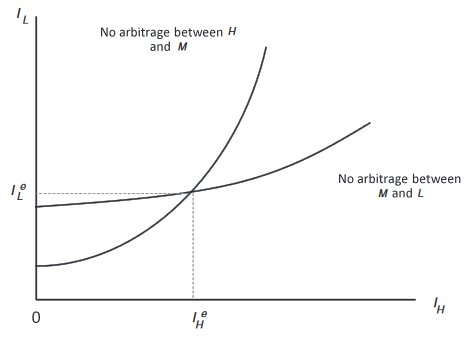
\includegraphics{HLE_equilibrium.png}}
        \label{fig_equilibrium}
    \end{center}
\end{figure}

While Figure \ref{fig_equilibrium} depicts the determination of the two thresholds, $I_L$ and $I_H$, it does not illustrate the allocation of tasks to different types of skills (workers). We do this in Figure \ref{fig_allocation}, which can also be interpreted as a diagram showing ``relative effective demand'' and ``relative effective supply''. In particular, we write (\ref{task_model_no_arbitrage_between_m_and_h}) as follows:
\begin{equation}
    \label{task_model_allocation}
    \frac{1-I_H}{I_H-I_L} \frac{\alpha_M\left(I_H\right)}{\alpha_H\left(I_H\right)}=\frac{A_H H}{A_M M} .
\end{equation}
The right-hand side of this Equation corresponds to the relative effective supply of high to medium skills. The left-hand side, on the other hand, can be interpreted as the effective demand for high relative to medium skills. The left-hand side of (\ref{task_model_allocation}) is shown as the outer curve in Figure \ref{fig_allocation}. It is downward sloping as a function of $I_H$ (for a given level of $I_L$) since $\a_M\of{I_H} / \a_H\of{I_H}$ is strictly decreasing in view of Assumption \ref{task_model_ass_comparative_advantage}. Similarly, we rewrite (\ref{task_model_no_arbitrage_between_m_and_l}) as:
$$
\frac{I_H-I_L}{I_L} \frac{\alpha_L\left(I_L\right)}{\alpha_M\left(I_L\right)}=\frac{A_M M}{A_L L},
$$
for given $I_H$, and this expression has the same relative effective demand and supply interpretation. The left-hand side traces a downward sloping curve as a function of $I_L$ (for given $I_H$) and is shown as the inner curve in Figure \ref{fig_allocation}. Figure \ref{fig_allocation} does not determine the two thresholds simultaneously as Figure \ref{fig_equilibrium} does, since the dependence of the two curves on the other threshold is left implicit. Nevertheless, Figure \ref{fig_allocation} is helpful in visualizing the equilibrium because it shows how equilibrium tasks are partitioned between the three types of skills. We will return to this figure when conducting comparative static exercises.

\begin{figure}[H]
    \noindent\caption{Equilibrium allocation of skills to tasks.}
    \begin{center}
        \resizebox{0.7\textwidth}{!}{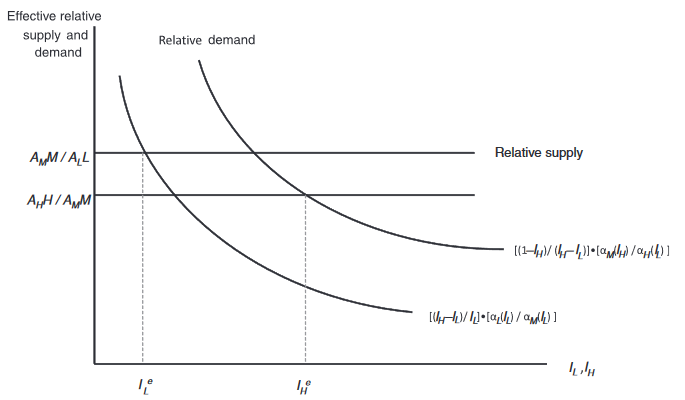
\includegraphics{HLE_allocation.png}}
        \label{fig_allocation}
    \end{center}
\end{figure}

\subsection{Special Cases}

\subsection{Comparative Statics}

\subsection{Task Replacing Technologies}

\subsection{Endogenous Choice of Skill Supply}

\subsection{Offshoring}

\subsection{Directed Technical Change}




\bibliography{\CiteReference}


\end{document}
